\defi{8.1} Sea $O \in \P$ y $\rho > 0$. Entonces una \textbf{circunferencia} $\C$ es el conjunto de puntos a una distancia $\rho$ de $O$. $O$ es el \textbf{centro} y $\rho$ el \textbf{radio}.

\tma{8.3} Una circunferencia corta a una recta en a lo sumo dos puntos.

\defi{8.4} Dada $\C$ una recta que corta en dos puntos se llama \textbf{secante}, que corta en un punto se llama \textbf{tangente} y que no corta se llama \textbf{exterior}. Si para un punto $X \in \P, d(O,X) > d(O,\rho)$ el punto es exterior, y si $d(O,X) < d(O, \rho)$ entonces es interior.

\tma{8.5} Sea $\C$ con centro $O$. Si $t$ es tangente a $\C$ en $P_t$, entonces $t \perp r_{O,P_t}$.

\defi{8.6} Sean $P, P'$ dos puntos tales que $O =  \m[P,P']$. Entonces, si los puntos están en $\C$, se denominan \textbf{diametralmente opuestos en $\C$}, y $[P,P']$ es un diámetro de $\C$.

\tma{8.7}/\defi{8.9} Dados tres puntos no alineados, entonces existe una única circunferencia                                                                                                                                                                                                                                                                                                                                                                                                                                                                                                                                                                                                                                                                                                                                                                                                                                                                                                                                                                                                                                                                                                                                                                                                                                                                                                                                                                                                                                                                                                                                                                                                                                                                                                                                                                                                                                                                                                                                                                                                                                                                                                                                                                                                                                                                                                                                                                                                                                                                                                                                                                                                                                                                                                                                                                                                                                                                                                                                                                                                                                                                                                                                                                                                                                                                                                                                                                                                                                                                                                                                                                                                                                                                                                                                                                                                                                                                                                                                                                                                                                                                                                                                                                                                                                                                                                                                                                                                                                                                                                                                                                                                                                                                                                                                                                                                                                                                                                                                                                                                                                                                                                                                                                                                                                                                                                                                                                                                                                                                                                                                                                                                                                                                                                                                                                                                                                                                                                                                                                                                                                                                                                                                                                                                                                                                                                                                                                                                                                                                                                                                                                                                                                                                                                                                                                                                                                                                                                                                                                                                                                                                                                                                                                                                                                                                                                                                                                                                                                                                                                                                                                                                                                                                                                                                                                                                                                                                                                                                                                                                                                                                                                                                                                                                                                                                                                                                                                                                                                                                                                                       que pase por estos puntos, la \textbf{circunferencia circunscrita}.

\cor{8.8} Dos circunferencias tienen a lo sumo dos puntos en común. Si sólo tienen un punto en común se llaman \textbf{tangentes}.

\importante \tma{8.10} Sean $\C, \C'$ con centros $O, O'$ y radios $\rho, \rho'$ respectivamente. Si las dos circunferencias cortan en dos puntos, entonces se cumplen las siguientes desigualdades:
$$OO' < \rho+\rho' \quad \rho < OO'+\rho' \quad \rho' < OO' + \rho$$
Y si las circunferencias son tangentes, entonces se verifica una de estas igualdades:
$$OO' = \rho+\rho' \quad \rho = OO'+\rho' \quad \rho' =   OO' + \rho$$      

\tma{8.11} Sea $\C$ con centro $O$ y sean $\triangle PXY$ y $\triangle P'XY$ dos triángulos con vértices en $\C$ y $P, P', O$ están en el mismo semiplano determinado por $r_{XY}$. Si $X$ e $Y$ no son diametralmente opuestos, entonces $\measuredangle P = \measuredangle P' = \frac{1}{2}\measuredangle O$
\begin{figure}[H]
	\centering
	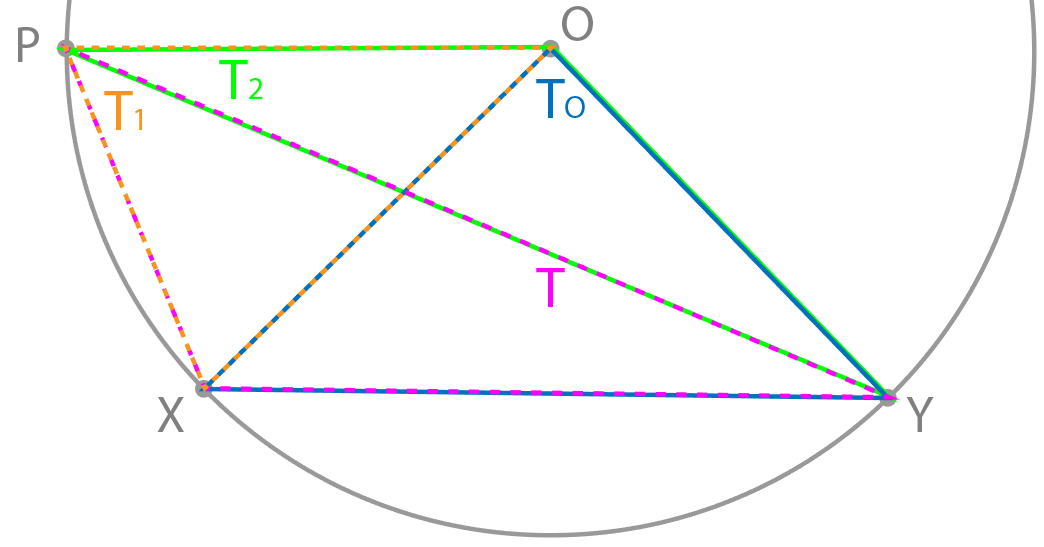
\includegraphics[width=7.5cm]{figuras/8-10.png}
	\vspace{-1em}
\end{figure}
\obligatorio\dem{Sea $\pazocal{T} = \triangle PXY$ y $\pazocal{T}_O =\triangle OXY$. Construimos también $\pazocal{T}_1 = \triangle POX$ y $\pazocal T_2 = \triangle POY$, isósceles, de modo que $\measuredangle_{\pazocal{T}_1} X = \measuredangle_{\pazocal{T}_1} P $ y $\measuredangle_{\pazocal{T}_2} Y = \measuredangle_{\pazocal{T}_2} P$. Como la suma de los ángulos de $\pazocal{T}_1$ y $\pazocal{T}_2$ es llano, entonces
$$2\measuredangle_{\pazocal{T}_1} P = \pi - \measuredangle_{\pazocal{T}_1} O \qquad 2\measuredangle_{\pazocal{T}_2} P = \pi - \measuredangle_{\pazocal{T}_2} O$$
Vamos a suponer ahora que $\measuredangle_{\pazocal{T}} P = \measuredangle_{\pazocal{T}_1} P-\measuredangle_{\pazocal{T}_2} P$. Para $2\measuredangle_{\pazocal{T}} P$ entonces se cumple que 
$$2\measuredangle_{\pazocal{T}} P = 2\measuredangle_{\pazocal{T}_1} P-2\measuredangle_{\pazocal{T}_2} P = \measuredangle_{\pazocal{T}_2}O-\measuredangle_{\pazocal{T}_1} O = \measuredangle_{\pazocal{T}_O} O = \measuredangle O$$
La misma demostración sucede para  $\measuredangle_{\pazocal{T}} P = \measuredangle_{\pazocal{T}_1} P+\measuredangle_{\pazocal{T}_2} P$ y  $\measuredangle_{\pazocal{T}} P = \measuredangle_{\pazocal{T}_2} P-\measuredangle_{\pazocal{T}_1} P$
} 

\defi{8.13} Sea $\C$ con centro $O$ y radio $\rho$. Se denomina \textbf{inversión} del plano con respecto a $\C$ a una aplicación $\iota_\C: \P- \{O\}\rightarrow \P-\{O\}$ que a cada punto $P$ le hace corresponder otro punto $\iota_\C(P)$ tal que $O, P, \iota_\C(P)$ están alineados, $O\not\in [P, \iota_\C(P)]$ y se verifica que 
$$OP\cdot O_{\iota_\C}(P) = \rho^2$$
Esta aplicación verifica que 
\begin{itemizex}
	\item $\iota_\C\circ \iota_\C(P) = P$ para todo $P\in \P -{O}$.
	\item Para todo $P \in \C$ se cumple $\iota_\C(P) = P$. A todo punto fuera del circulo, $\iota_\C$ lo manda dentro, y viceversa.
	\item Si $r$ pasa por $O$, $\iota_\C(r-\{O\}) = r-\{O\}$.
\end{itemizex}
\begin{figure}[H]
	\centering
	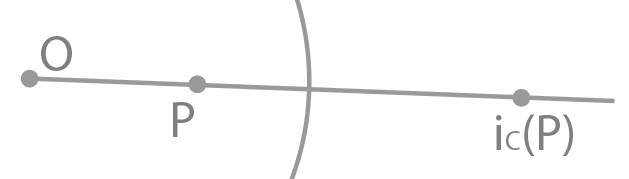
\includegraphics[width=7.5cm]{figuras/8-15.png}
	\vspace{-1em}
\end{figure}
\tma{8.16/8.17} Sea $\C$ y $P\in \P$. Sean $a, b$ rectas que cortan a $P$ y secantes a $\C$. Sean $A_1$ y $A_2$ los puntos de corte de $a$ con $\C$ y $B_1, B_2$ los de $b$ con $\C$. Entonces se verifica que 
\[PA_1\cdot PA_2 = PB_1 \cdot PB_2  \] 
Si $a$ es tangente, entonces 
\[PA^2 = PB_1 \cdot PB_2  \] 
Ese producto, por tanto, es invariante de la recta, y se denomina \textbf{potencia de $P$ con respecto a $\C$}.

\tma{8.18} Sea $\C$ de radio $\rho$ y centro $O$.
\begin{itemizex}
	\item Sea $\C'$ una circunferencia de centro $O'$ que pasa por $O$, entonces $\iota_\C(\C'-\{O\})$ es una recta ortogonal a $r_{O,O'}$. Sea $r$ que no pasa por $O$, entonces $\iota_\C(r) = \C'-\{O\}$, donde $\C'$ es una circunferencia que pasa por $O$.
	\item Si $\C'$ no pasa por $O$ entonces $\iota_\C(\C')$ es otra circunferencia que no pasa por $O$. Si $O$ es exterior a $\C'$ entonces $\iota_\C(\C')$ es la imagen de $\C'$ por la homotecia de centro $O$ y razón $\rho^2/t$, donde $t$ es la potencia de $O$ con respecto a $\C'$. Si $O$ es interior a $\C'$ entonces $\iota_\C(\C') = \sigma_O \circ \eta_{O,\rho^2/t}(\C)$.
\end{itemizex}